\setAuthor{Tundmatu autor}
\setRound{lahtine}
\setYear{2008}
\setNumber{G 5}
\setDifficulty{4}
\setTopic{Dünaamika}

\prob{Kuulike}
Venimatu ja kaalutu niidi otsa kinnitati kuulike.
Niit viidi horisontaalasendisse ja lasti lahti. Kuulikese kiiruse vertikaalne komponent
hakkab esialgu suurenema, kuid teatud hetkest alates vähenema. Millise nurga moodustab niit vertikaalsihiga ajahetkel, kui kuulikese kiiruse vertikaalne komponent on
maksimaalne?

\hint
Kuulikese kiirus on leitav energia jäävuse seadusest. Edasi taandub ülesanne ekstreemumpunkti leidmisele.

\solu
Olgu $\alpha$ nurk vertikaali ja varda vahel ning l niidi pikkus. Energia jäävuse seadusest
$v^2 = 2gl \cos \alpha$, millest kiiruse vertikaalkomponendi ruut
\[
v_{y}^{2}=2 g l \cos \alpha \sin ^{2} \alpha=2 g l \cos \alpha\left(1-\cos ^{2} \alpha\right).
\]
Tähistades $\cos \alpha = y$, saame $v_y^2$ maksimumi tingimuse, kui võtame sellest tuletise $y$ järgi:
\[
\frac{\D v_{y}^{2}}{\D y}=2 g l\left( 1-3 y^{2}\right)=0,
\]
millest $y = 1/ \sqrt 3$ ja $\alpha = \arccos \left( 1/ \sqrt 3\right) \approx \ang{55}$.

\vspace{0.5\baselineskip}

\begin{wrapfigure}{r}{0.3\textwidth}
	\begin{center}
		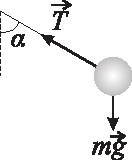
\includegraphics[width=0.95\linewidth]{2008-lahg-05-lah}
	\end{center}
\end{wrapfigure}
\emph{Alternatiivne lahendus}\\
Ülesandes on öeldud, et kuulikese kiiruse vertikaalne komponent
hakkab esialgu suurenema, kuid teatud hetkest alates vähenema.
See tähendab seda, et kuulikese kiirenduse vertikaalne komponent oli alguses positiivne ning pärast muutus negatiivseks. Järelikult hetkel, kui kiiruse vertikaalne komponent on maksimaalne, on kiirenduse vertikaalne komponent null. Seega vaadeldaval
hetkel võrdub kuulikese raskusjõu ja niidi tõmbejõu vertikaalsete
projektsioonide summa nulliga ehk siis
\begin{equation} \label{2008-lahg-05:eq1}
mg = T \cos \alpha.
\end{equation}
Kuuli kesktõmbekiirendus on $a_n = v^2/l$, kus $l$ on niidi pikkus. Seega Newtoni II
seaduse põhjal
\begin{equation} \label{2008-lahg-05:eq2}
m\frac{v^2}{l} = T - mg \cos \alpha.
\end{equation}
Energia jäävuse seadusest
\begin{equation} \label{2008-lahg-05:eq3}
v^2 = 2gl \cos \alpha.
\end{equation}

Asendades võrdusesse (\ref{2008-lahg-05:eq2}) avaldised $T$ ja $v^2$
jaoks võrdustest (\ref{2008-lahg-05:eq1}) ja (\ref{2008-lahg-05:eq3}) saame
\[
\frac{m \cdot 2 g l \cos \alpha}{l}=\frac{m g}{\cos \alpha}-m g \cos \alpha,
\]
millest
\[
\frac{1}{\cos \alpha}-\cos \alpha=2 \cos \alpha \quad \Rightarrow\quad \cos \alpha=\frac{1}{\sqrt{3}}.
\]
Siit $\alpha = \arccos \left( 1/ \sqrt 3\right) \approx \ang{55}$.
\probend